Mark Hall, Eibe Frank, Geoffrey Holmes, Bernhard Pfahringer, Pe- ter Reutemann, Ian H. Witten (2009); The WEKA Data Mining Software: An Update; SIGKDD Explorations, Volume 11, Issue 1.
pag 215 manual_weka (radomizacao)

**Coloca o desvio padrão tb na comparação das medidas.
\begin{figure}[!htb] \centering 
  \centering
  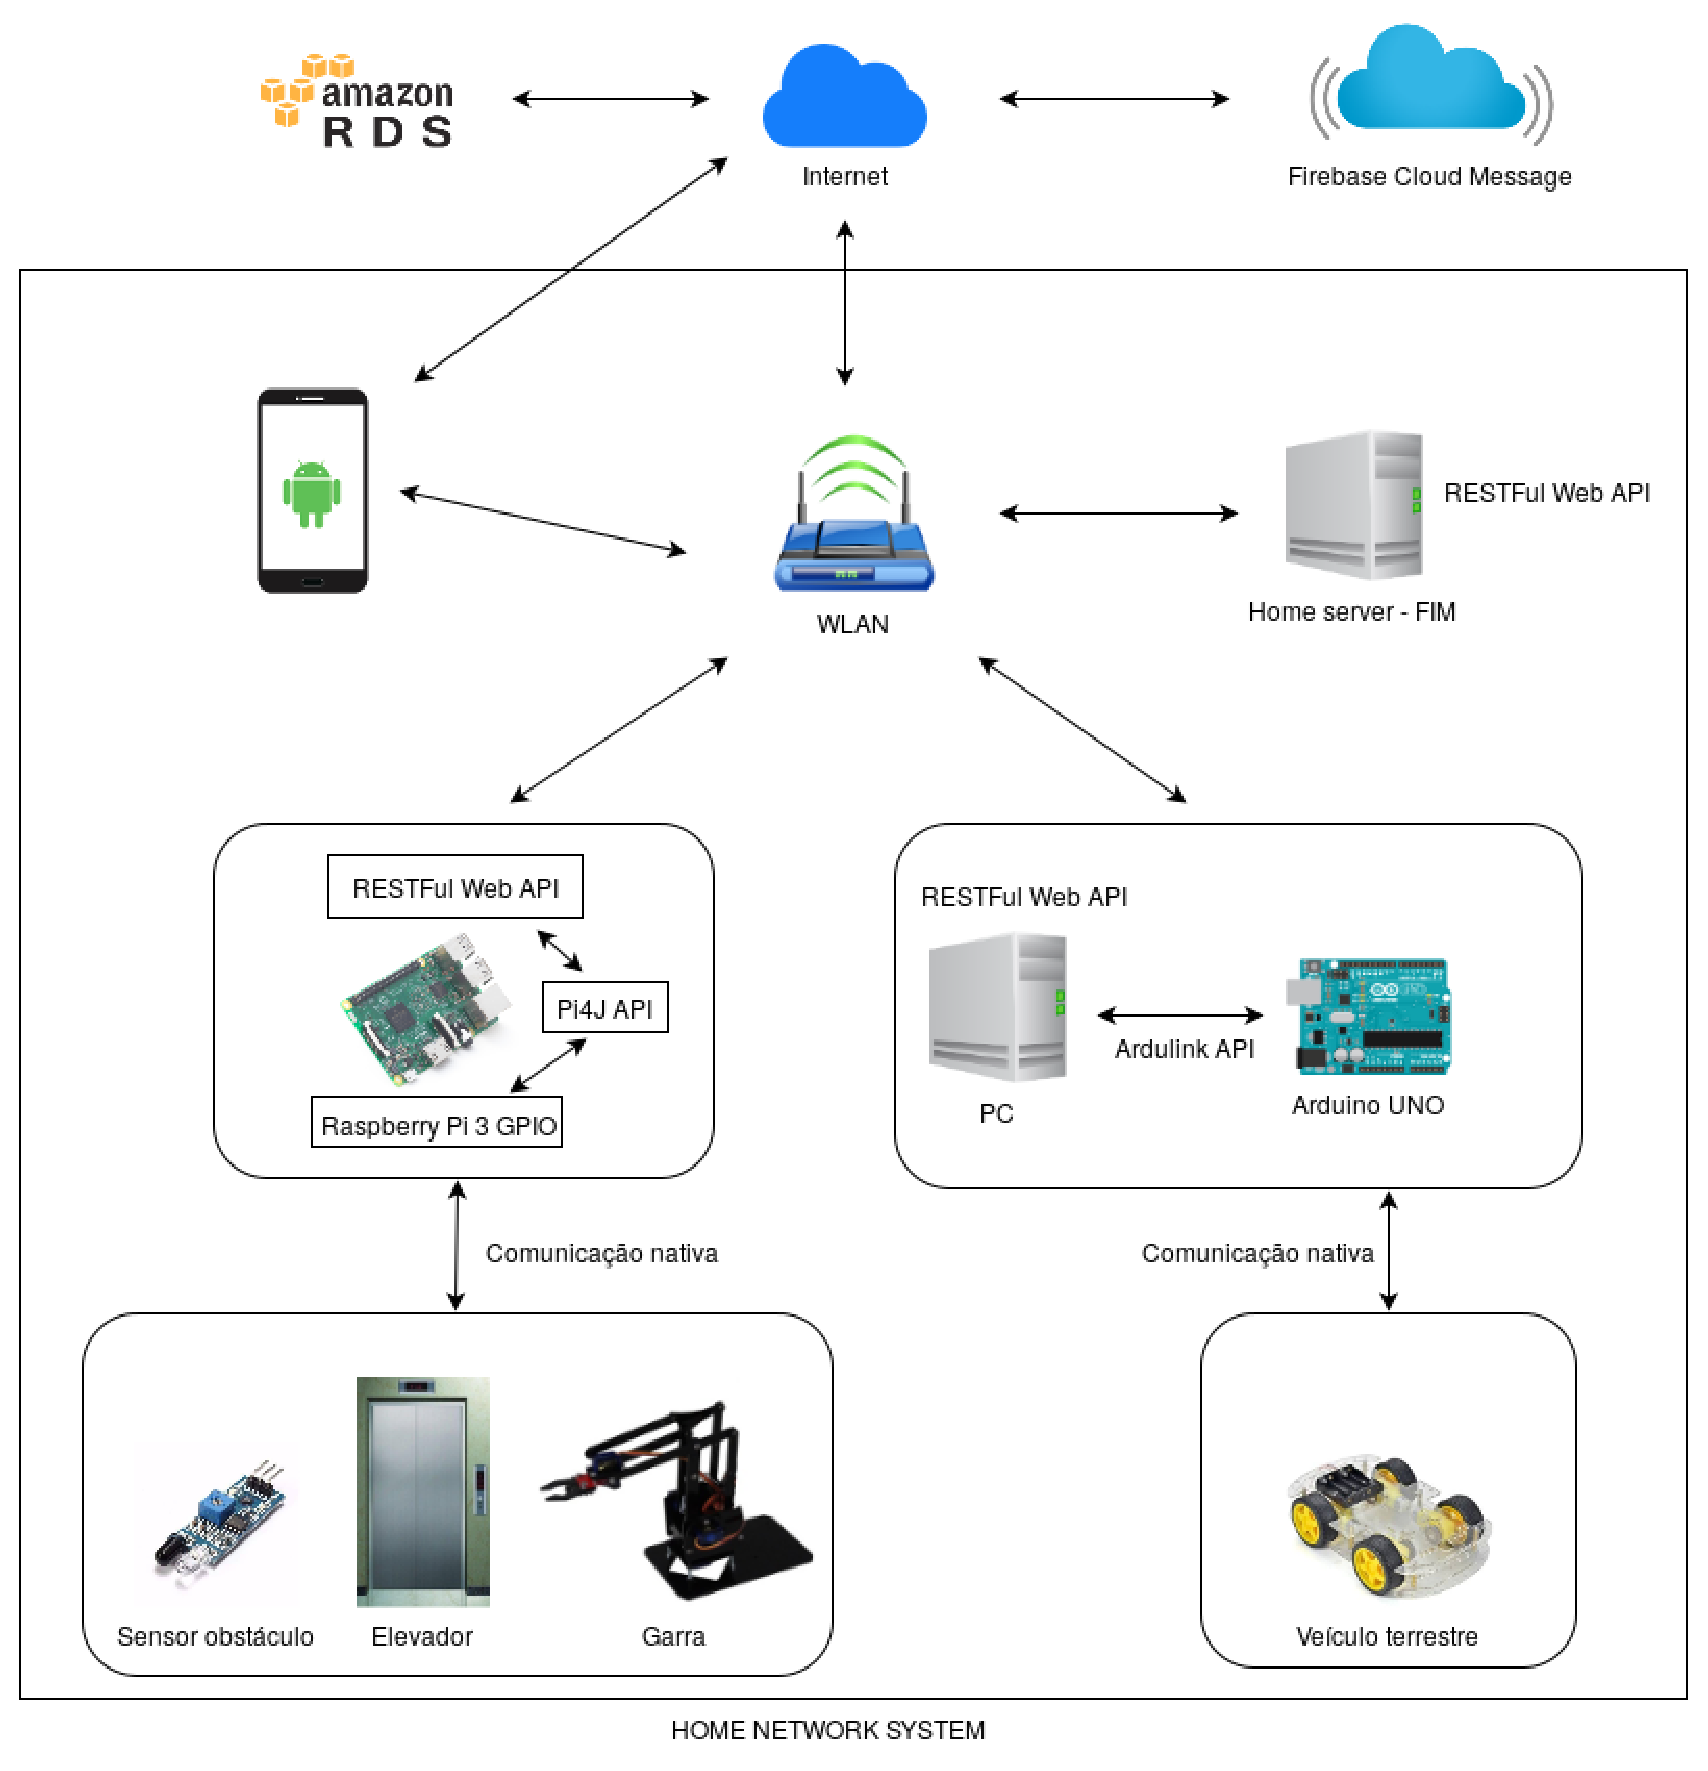
\includegraphics[width=0.8\columnwidth]{cenario} 
  \caption{Modelo do HNS utilizado neste trabalho.} 
  \label{fig:hnsworkmodel}
\end{figure}

**Ve se da para usar o Experimenter ou o Evaluation no fonte.


**VE SE DA TEMPO PARA RODA UM OUTRO CLASSIFICADOR E VERIFICAR OS RESULTADOS**
**trees.SimpleCart**
trees.DecisionStump
functions.SMO
trees.BFTree
trees.LMT
trees.FT
**ver se dar tempo de gerar curva roc(verifdicar o motivo da roc, é viavel para este cenário) e precision e recall dos resultados dos 3 modelos**

MOTIVO:
escolher os melhores parametros para o modelo em questão, neste caso, rede neural.

 machine learning and statistics, feature selection, also known as variable selection, attribute selection or variable subset selection, is the process of selecting a subset of relevant features (variables, predictors) for use in model construction. Feature selection techniques are used for three reasons:

        simplification of models to make them easier to interpret by researchers/users,[1]
        shorter training times,
        enhanced generalization by reducing overfitting[2](formally, reduction of variance[1])



Procedimentos utilizados - experimento:
-gera uma plotMatriz dos dados do dataset
-verifica quais dados poderiam ser melhor separados por uma curva(par a par)

-neste caso, visualmente são esse abaixo:
t_num_width e t_num_diameter
(quem não tem width, tem diameter e vice e versa)
t_num_mass e t_num_width

-testa com alguma combinação distinta dos parâmetros acima
t_num_width, t_num_mass, t_num_diameter 

-Verifica a generalização utilizando técnicas estaitisticas, tais como, stratifyed-k-crossvalidation e/ou randomized-holdout

-escolhe o melhor modelo baseado no que você quer do modelo, neste caso o que tiver melhor recall, seguido de accuracy. POIS É MELHOR ERRAR DIZENDO QUE É, DO QUE ERRAR DIZENDO QUE NÃO É.

-gera um classificador com todo o dataset verificado na etapa anterior.
-testa esse classificador com um dataset distinto do anterior.
-DEMONSTRA OS RESULTADOS E COMPARA COM OS TESTES ANTERIORES.